\documentclass[12pt, a4paper]{report}
\usepackage{geometry}
\usepackage{graphicx}
\usepackage{float}
\usepackage{subfigure}
\usepackage{booktabs}
\geometry{left=2cm,right=2cm}
\title{COVID-19 and Economics Indicators in the UK}
\author{Siyu YANG}
\date{}

\begin{document}
\maketitle

\section{Research Questions}
This report is aimed to research on the associations between the severity of COVID-19 and some important 
economics indicators in the UK. More specifically, this report will answer the following questions:
1) Which COVID-19 severity indicator(s) and which economics indicator(s) have high and significant relationships?
2) And how these severity indicator(s) impact these economics indicator(s) exactly?


\section{Datasets}
\subsection{COVID-19 Datasets (updated on 05-02-2021)}
The following three COVID-19 datasets contain the number of positive cases, deaths, and patients admitted to hospitals, 
respectively. Each dataset includes the newly-add number and cumulative number.\par
\noindent
1) Positive cases by spicemen date
\footnote[1]{https://coronavirus.data.gov.uk/details/cases};\par
\noindent
2) Deaths with COVID-19 within 28 days of positive test by date of death
\footnote[2]{https://coronavirus.data.gov.uk/details/deaths};\par
\noindent
3) Patients admitted to hospital
\footnote[3]{https://coronavirus.data.gov.uk/details/healthcare}\par

\subsection{Economic indicators (updated in November 2020)} 
The following two datasets contain the data of five economics indicators: monthly GDP, service index, 
production index, construction index, and unemployment rate.\par
\noindent
1) Monthly GDP and components index (seasonally adjusted)
\footnote[4]{https://www.ons.gov.uk/economy/grossdomesticproductgdp/};\par
\noindent
2) Unemployment rate (aged 16 and over, seasonally adjusted)
\footnote[5]{https://www.ons.gov.uk/employmentandlabourmarket/peoplenotinwork/unemployment/}

\subsection{Stock Index (updated on 05-02-2021)}
1) FTSE 100 Index;\par
\noindent
2) FTSE All-Share Index
\footnote[6]{Source: Capital IQ}


\section{Methodology and Results}
1. To answer the first research question, correlations between COVID-19 severity indicators
and economics indicators(including stock index) have been examined:

\begin{figure}[H]
\centering
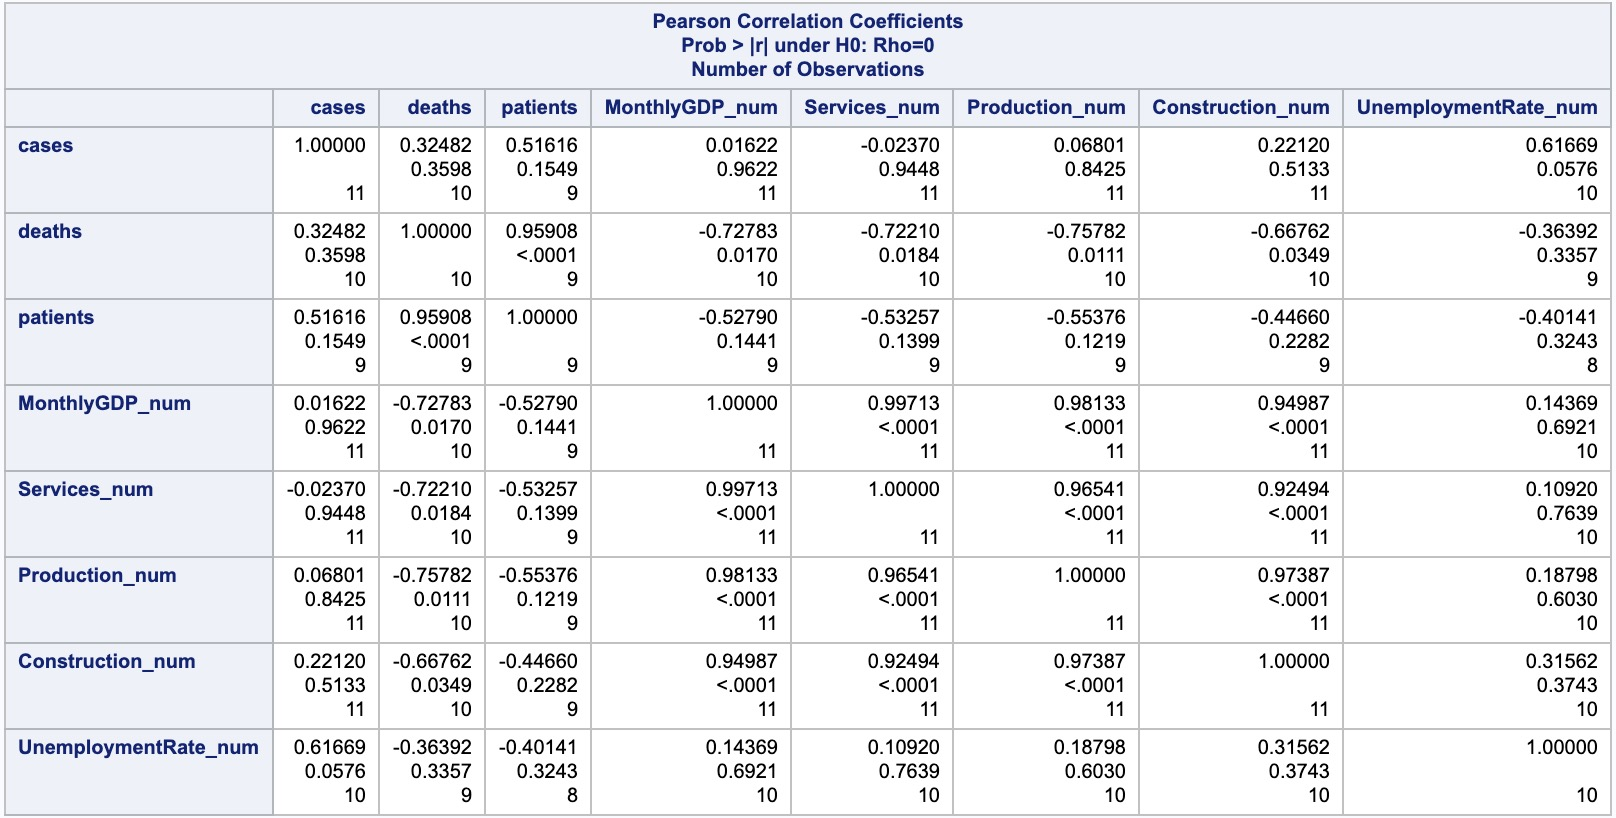
\includegraphics[width=15cm]{corr_economics_new.jpg}
\caption{Correlation Matrix Economics Indicators (new)}
\label{Fig1. Corrlation Matrix 1}
\end{figure}

\begin{figure}[H]
\centering
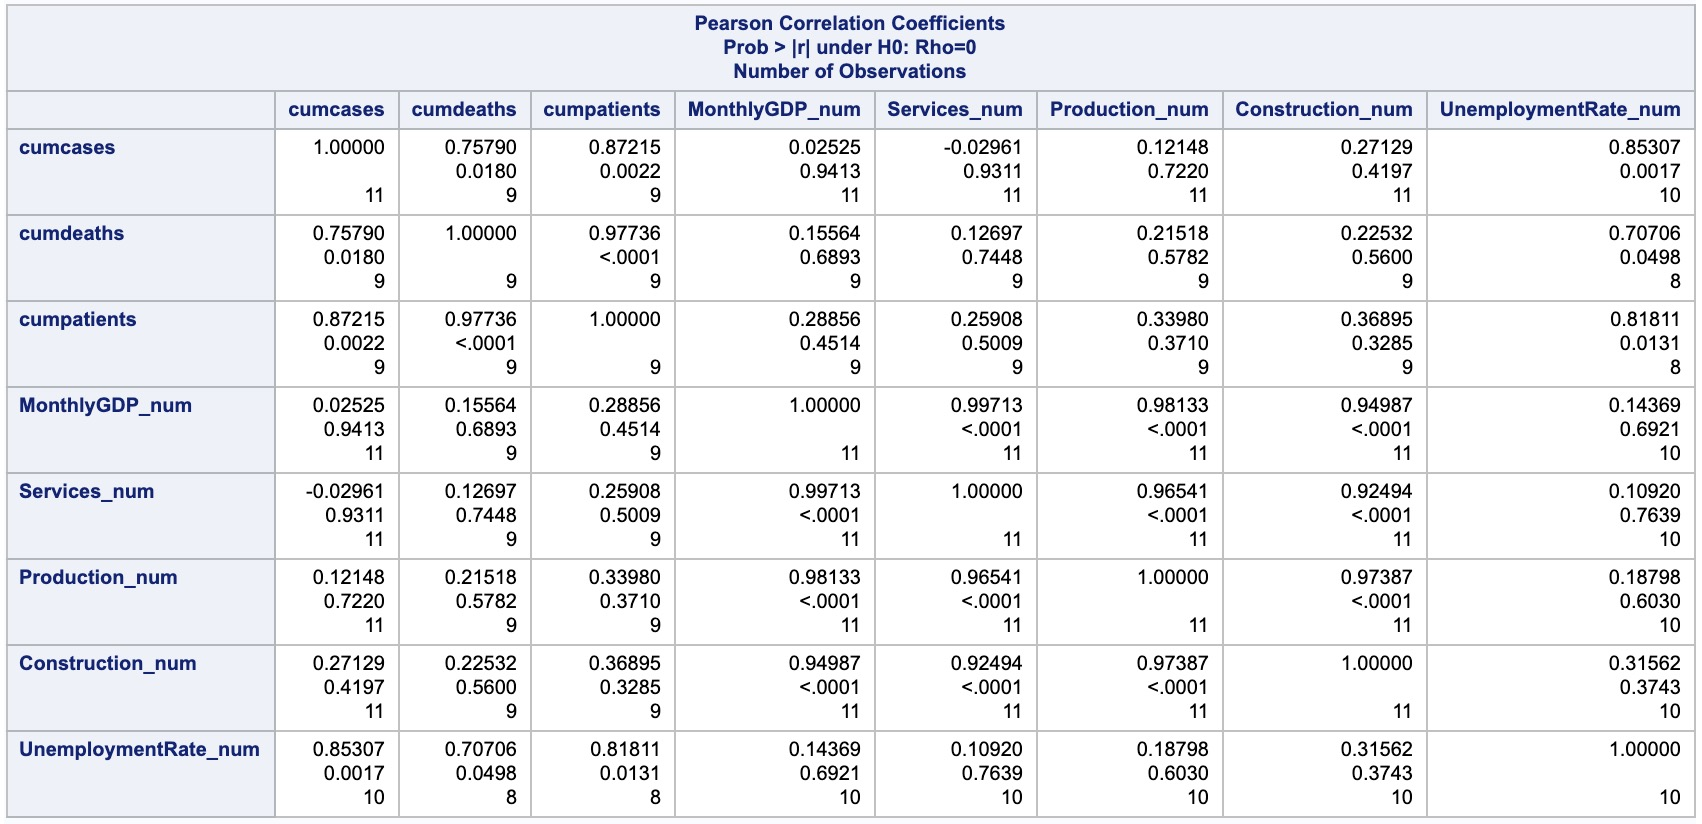
\includegraphics[width=15cm]{corr_economics_cum.jpg}
\caption{Corrlation Matrix Economics Indicators (cum)}
\label{Fig2. Corrlation Matrix 1}
\end{figure}

\begin{figure}[H]
\centering
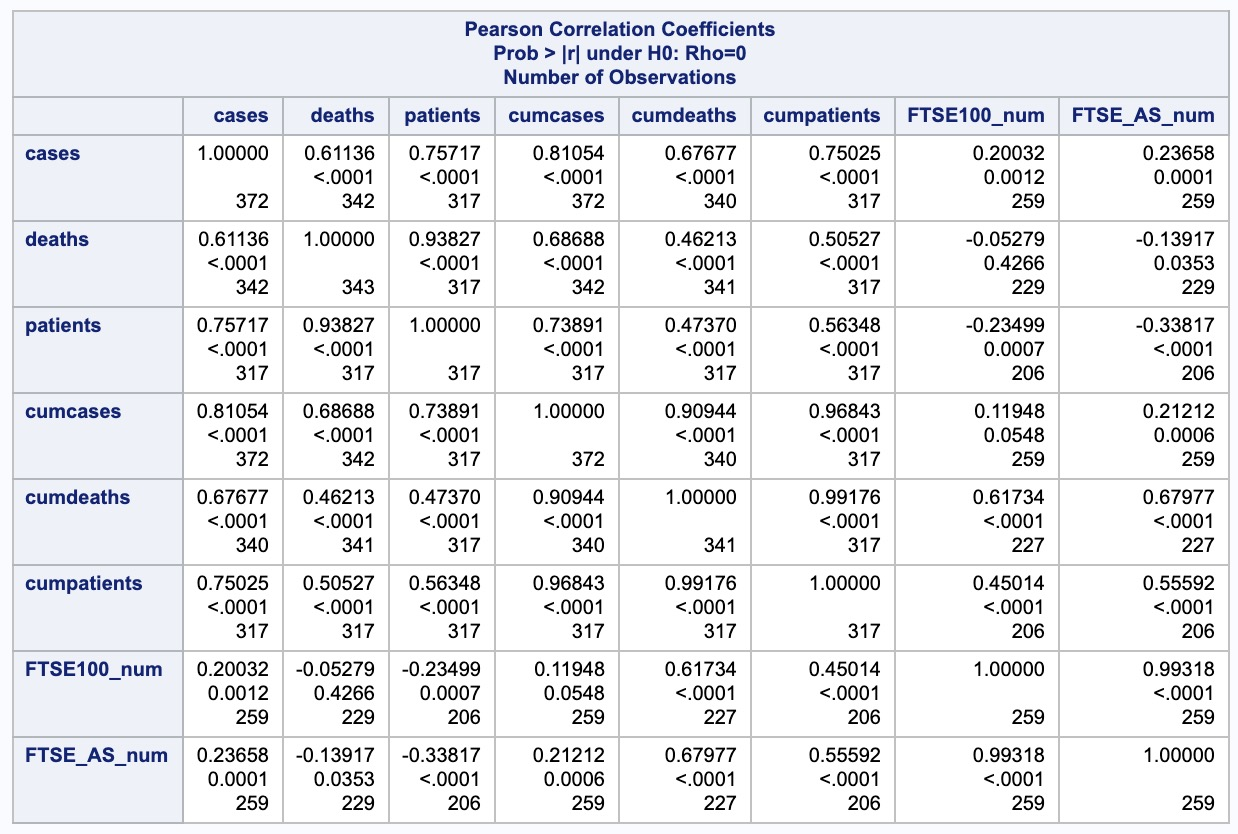
\includegraphics[width=15cm]{corr_FTSE.jpg}
\caption{Correlation Matrix FTSE}
\label{Fig2. Corrlation Matrix 2}
\end{figure}

\noindent
From Fig.1, we can see that only 'deaths' have significant and relatively high correlations with monthly GDP and 
components indexes; Fig.2 tells us that all three cumulative COVID-19 indicators have significant and high 
correlations with unemployment rate; Fig.3 shows that 'cumdeaths' and 'cumpatients' have significant and relatively
high correlations with two stock indexes whereas 'cases' and 'patients' have significant correlations with 
stock indexes, 'deaths' and 'cumcases' also have significant correlations with FTSE All Share.\par
\hspace*{\fill}

\noindent
2. As for the second question, regression analysis is implemented to further explore how COVID-19 indicators impact 
economics indicators. Only highly and significantly correlated variables are chosen to perform regression analysis.\par
\noindent
1) Table1 is the summary of regression analysis (with only one parameter) on COVID-19 indicators and economics indicators (including
stock indexes);\par
\noindent
2) This report also treis to build regression models to predict the stock indexes with multiple variables. 
Table2 is the summary of some models with relatively good performance. 

\begin{table}[H]
    \begin{center}
    \begin{tabular}{llcccc}
        \toprule
        Y&X&Coef&Intercept&p&R-square\\
        \midrule
        Monthly GDP&Deaths&-0.00073&93.31&0.017&0.53\\
        Service Index&Deaths&-0.00068&92.62&0.018&0.52\\
        Production Index&Deaths&-0.00074&96.14&0.011&0.57\\
        Condtruction Index&Deaths&-0.0014&95.28&0.035&0.45\\
        Unemployment Rate&CumCases&1.09e-6&4.05&0.0017&0.73\\
        Unemployment Rate&CumDeaths&2.04e-5&3.73&0.050&0.50\\
        Unemployment Rate&CumCases&7.14e-6&3.62&0.013&0.67\\
        \midrule
        FTSE100&CumDeaths&0.015&5634.58&<0.0001&0.38\\
        FTSE100&CumPatients&0.0038&5736.78&<0.0001&0.20\\
        FTSE All Share&CumDeaths&0.010&3080.48&<0.0001&0.46\\
        FTSE All Share&CumPatients&0.0030&3114.20&<0.0001&0.31\\
        \bottomrule
    \end{tabular}
    \caption{Regression Analysis}
    \end{center}
\end{table}

\begin{table}[H]
    \begin{center}
    \begin{tabular}{llcccccc}
        \toprule
        Y&X1&Coef1&X2&Coef2&Intercept&p&R-square\\
        \midrule
        FTSE100&cases&0.0480&patients&-0.1458&6.114.67&<0.0001&0.44\\
        FTSE100&cumcases&0.0020&cumpatients&-0.0029&5931.38&<0.0001&0.40\\
        FTSE100&cumdeaths&0.0314&patients&-0.1170&3428.90&<0.0001&0.54\\
        FTSE All Share&cases&0.0314&patients&-0.1170&3428.90&<0.0001&0.54\\
        FTSE All Share&cumcases&0.0013&cumpatients&-0.0014&3241.15&<0.0001&0.52\\
        FTSE All Share&cumdeaths&-0.0535&cumpatients&0.0209&5686.38&<0.0001&0.31\\
        \bottomrule
    \end{tabular}
    \end{center}
    \caption{Regression Models to Predict the Stock Indexes}
\end{table}

\section{Limitations}

\begin{appendix}
\end{appendix}
\end{document}